\section{Two-Party Tests}
\label{sec:two-party-test}

Two-Party tests are the normal telephone calls between two participants.
User A calls another user (perhaps User B) who has to be registered, makes a phone call and hangs up.

As a \texttt{sip} dialog, the scenario looks as follows:
\begin{figure} [!ht]
\centering
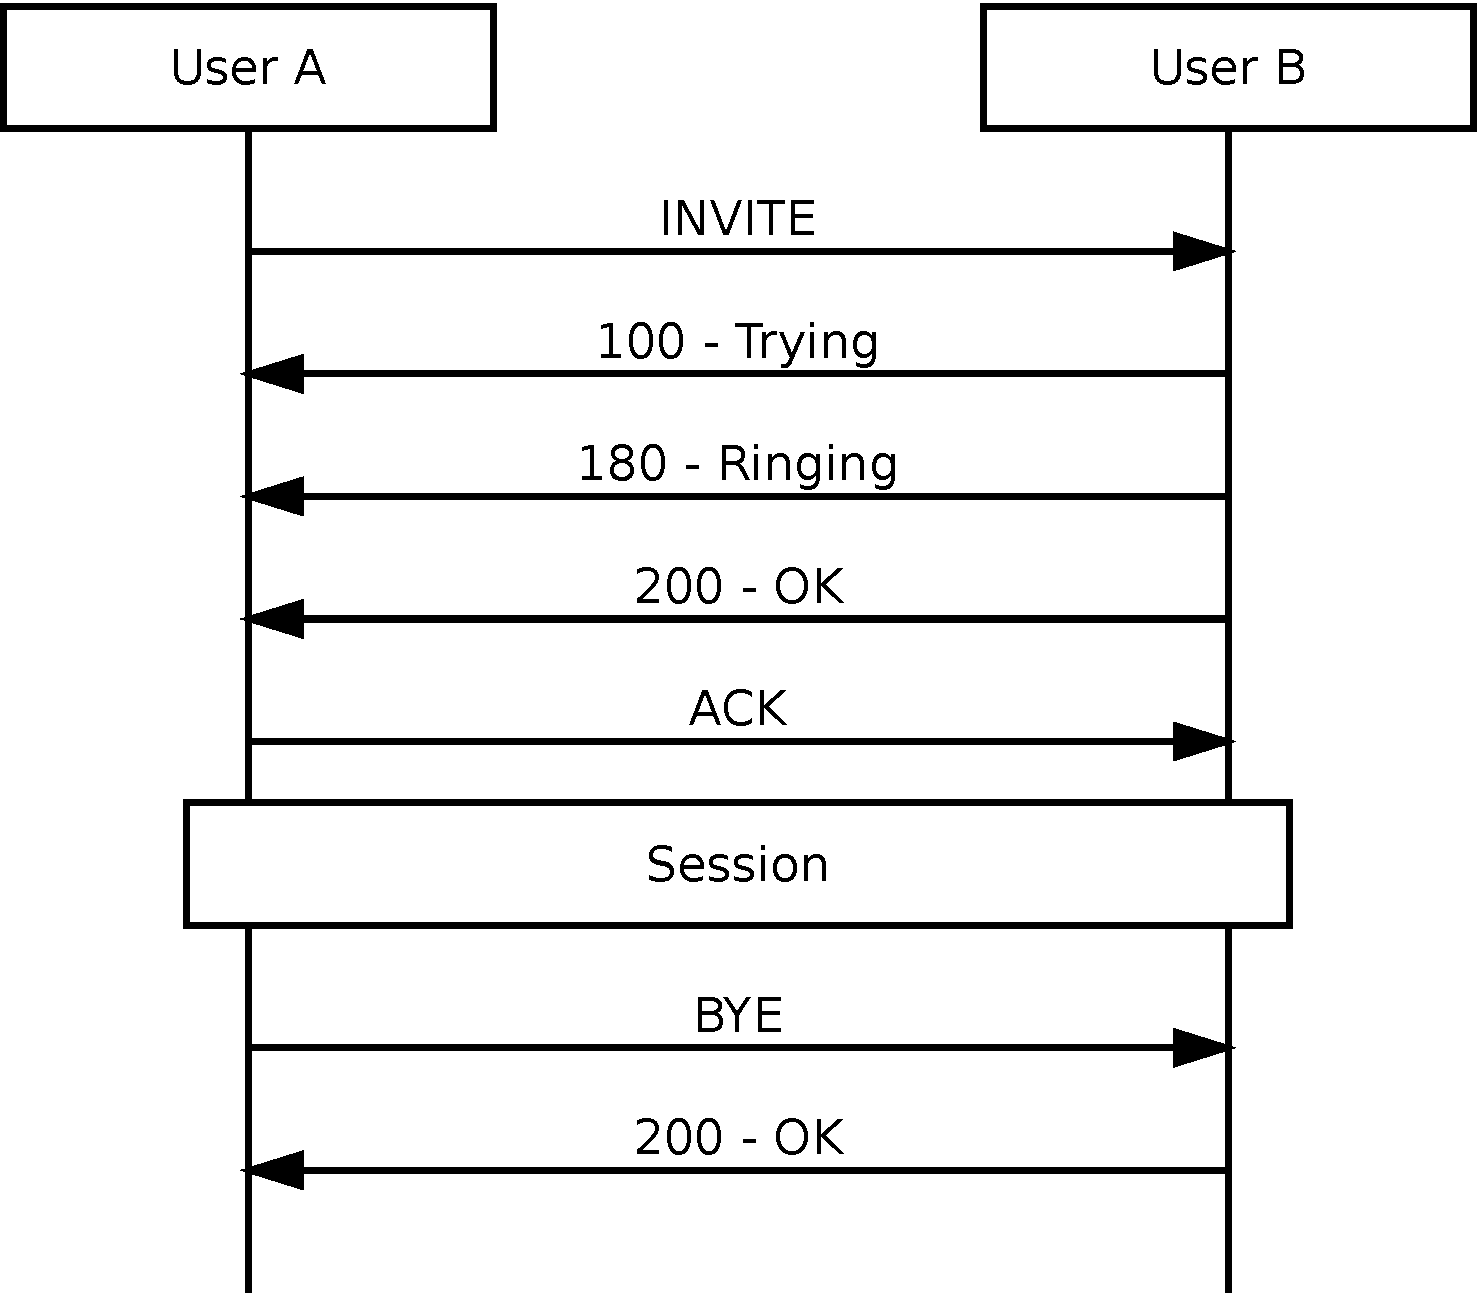
\includegraphics [width=10cm] {two-party-1}
\caption{SIP dialog of a two-party call}
\end{figure}
The original XML scenarios for sipp used to implement this are available in the appendix. \newpage

\begin{figure} [!ht]
\centering
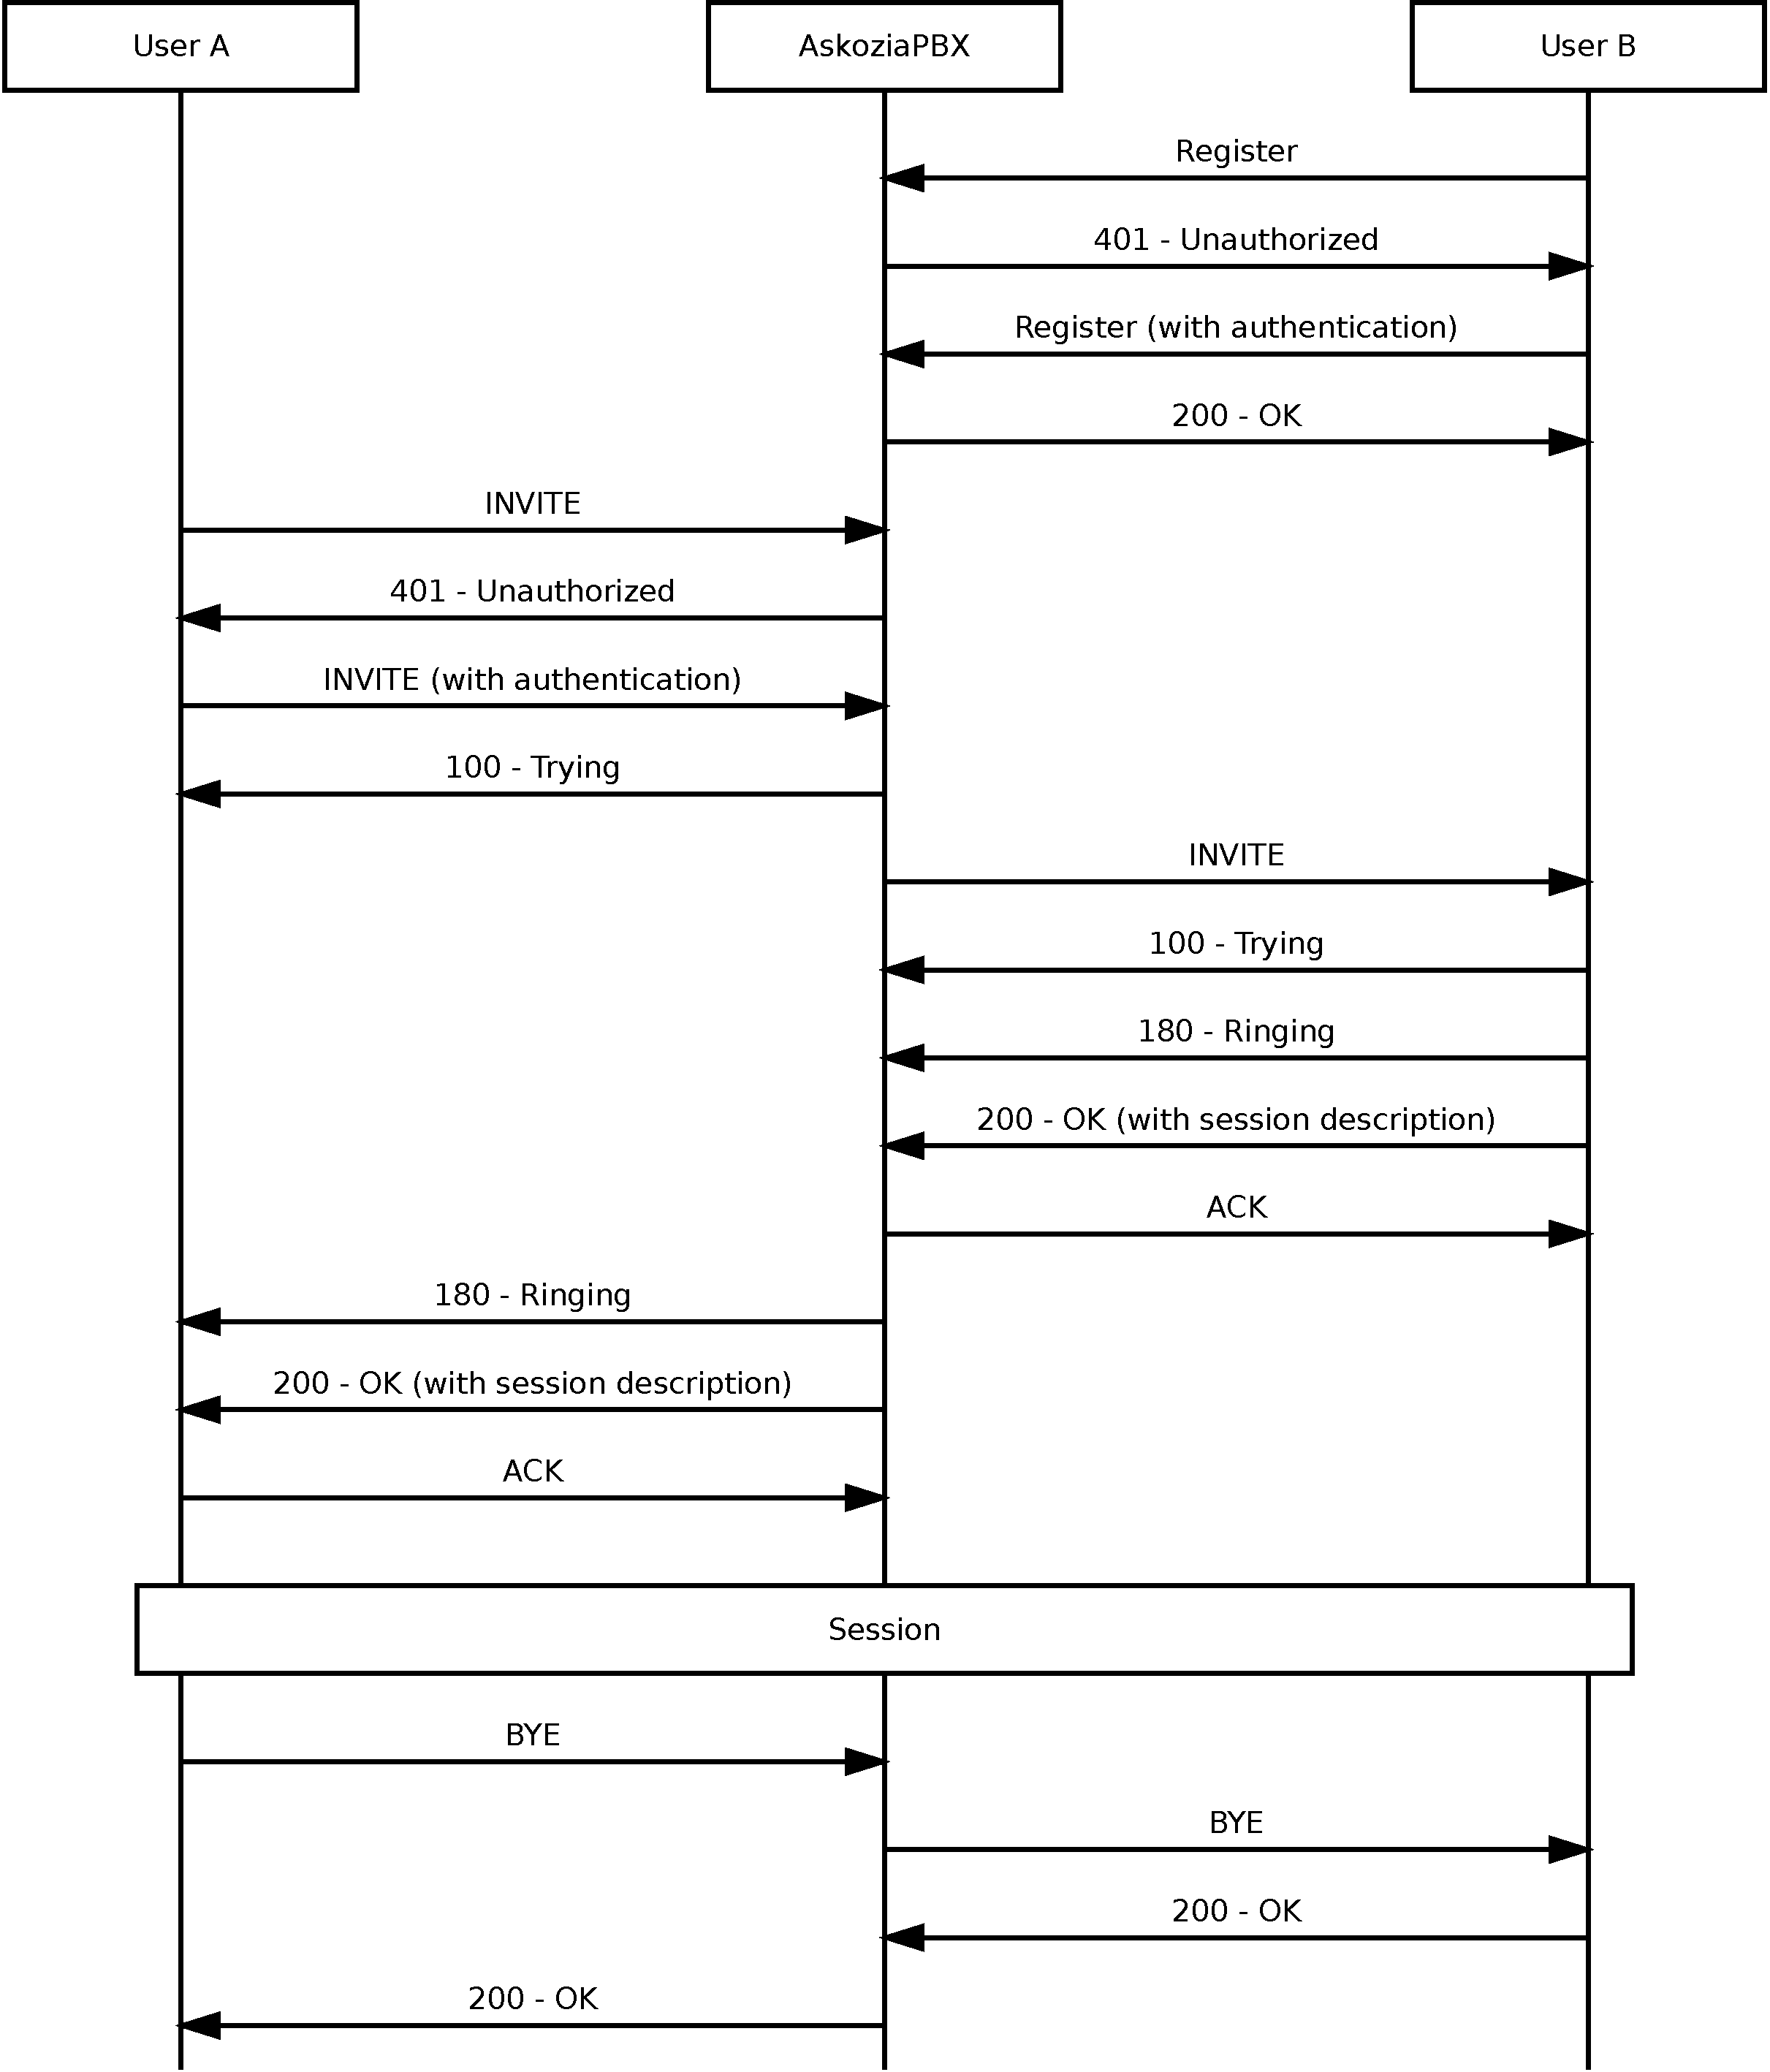
\includegraphics [width=15cm] {two-party-2}
\caption{Dialog of a two-party call}
\end{figure}

The next diagramm shows the process of a complete two-party test: \newpage
\begin{figure} [!ht]
\centering
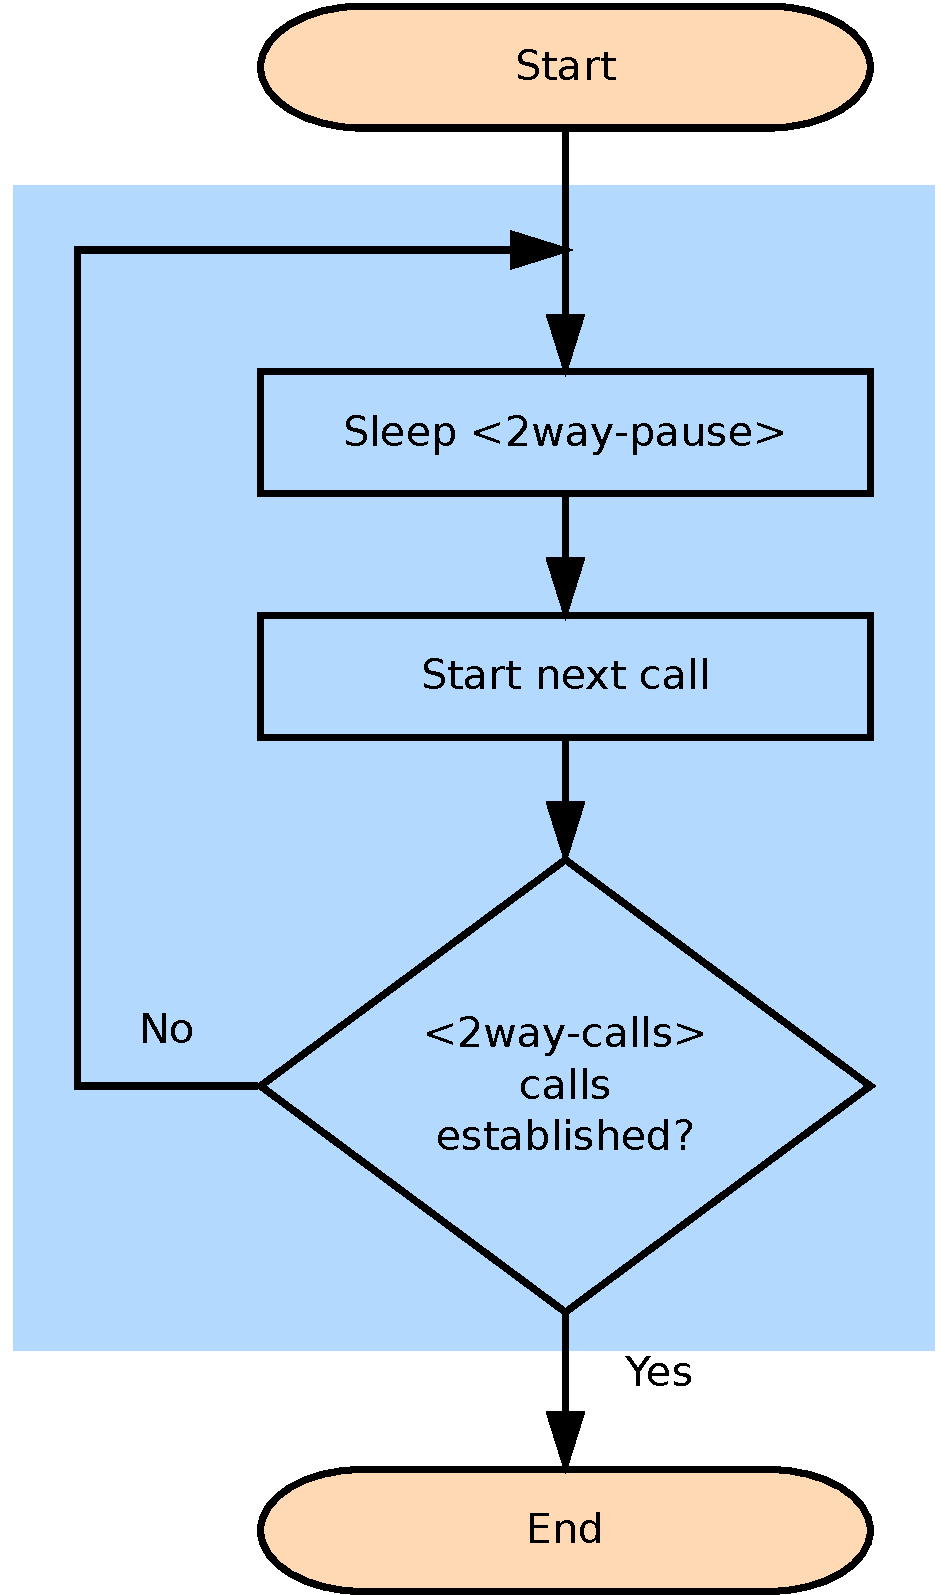
\includegraphics [width=5cm] {two-party-3}
\caption{Complete two-party test}
\end{figure}

The number of calls is increased step-by-step. After every call, the script waits for the specified pause
time to record the CPU load values. For executing two-party calls, the following sipp commands used.
You can inform yourself about the used parameters by reading the sipp manpage (the appendix contains the sipp manpage).
It is possible to change the used sip and rtp ports as well as the name of the csv files by using the developers parameters. 
For more information, please have a look at the appendix. In original call, the csv files are specified by their absolut path. 
\begin{lstlisting}[breaklines=true,label=code:twoway-invite,caption={sipp command for inviting User B} ]
REGISTER Command:
sipp -aa -inf 'Users_two-party.csv' -m $current_call -i $local_ip
  -p 5062 -mp 6030 -sf 'Register.xml' $ask_ip 2>&1

ACCEPT Command:
sipp -aa -inf 'Users_two-party.csv' -m $current_call -i $local_ip
  -p 5062 -mp 6030 -sf 'Accept.xml' -bg $ask_ip 2>&1 &

INVITE Command:
sipp -aa -inf 'Users_two-party.csv' -m $current_call -i $local_ip
  -p 5061 -mp 6020 -sf 'Invite.xml' $ask_ip 2>&1

De-REGISTER Command:
sipp -aa -inf 'Users_two-party.csv' -m $current_call -i $local_ip
  -p 5062 -mp 6030 -sf 'Deregister.xml' $ask_ip 2>&1
\end{lstlisting}

